
\newpage
\section{Question to Wolfgang}

The code solves the following manufactured solution problem
which originates in Dohrmann \& Bochev \cite{dobo04}: 
\begin{eqnarray}
u_x(x,y) &=& x+x^2 - 2xy+x^3 - 3xy^2 + x^2y \\
u_y(x,y) &=& -y-2xy+y^2 -3x^2y + y^3 - xy^2 \\
p(x,y) &=& xy+x+y+x^3y^2 - 4/3
\end{eqnarray}

The element pair I am using is $Q_1\times P_0$ (I know, but there is a good reason, I'll 
explain later, bear with me:).
The velocity and pressure fields are as follows:

\begin{center}
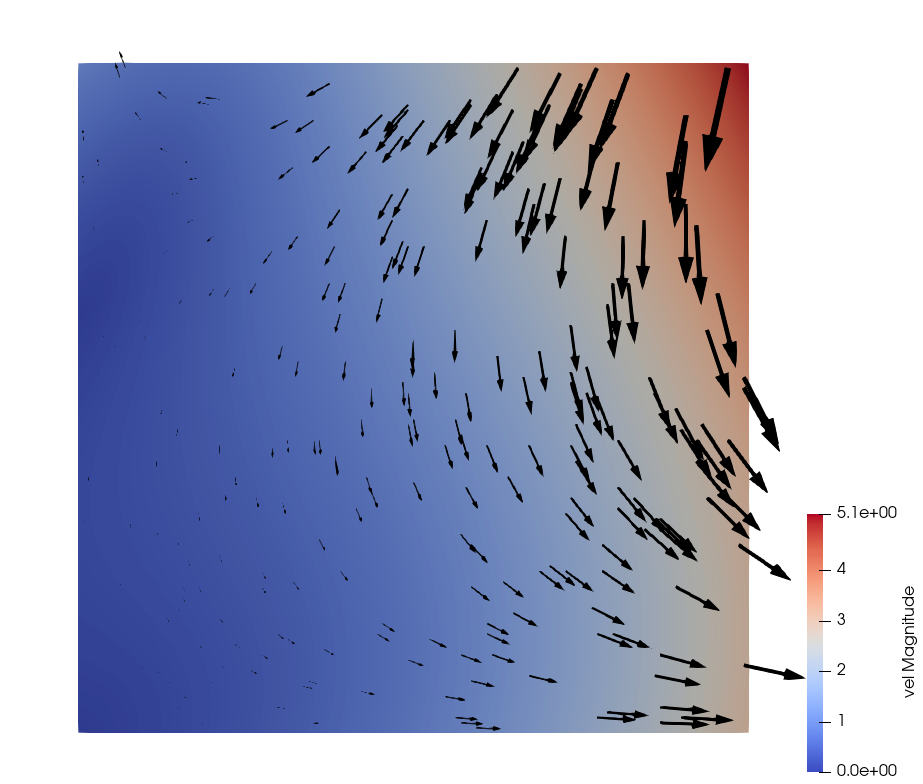
\includegraphics[width=7cm]{../results/exp09/vel.png}
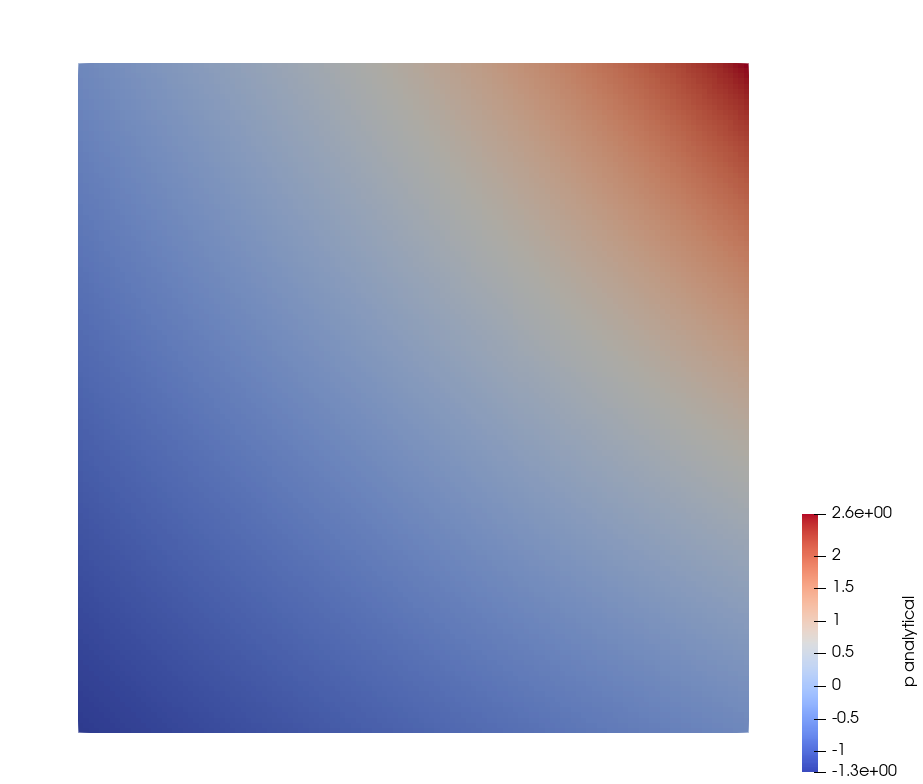
\includegraphics[width=7cm]{../results/exp09/press.png}
\end{center}

The analytical field is such that $\int_\Omega p dV= 0$.
As in our 2 previous papers, I solve the Stokes system (without 
any imposed constraint wrt zero pressure average) using a built-in direct solver
and later normalize the pressure to zero.

At this stage I must say that the same code running on the Donea \& Huerta manufactured
solution yields the right error rates for velocity and pressure, with a zest of pressure 
checker board modes.

If I run this new benchmark I find that the velocity is visually plagued by imperfections, 
that its error rate convergence is all over the place and that the pressure field 
is so 14 orders of magnitude off:

\begin{center}
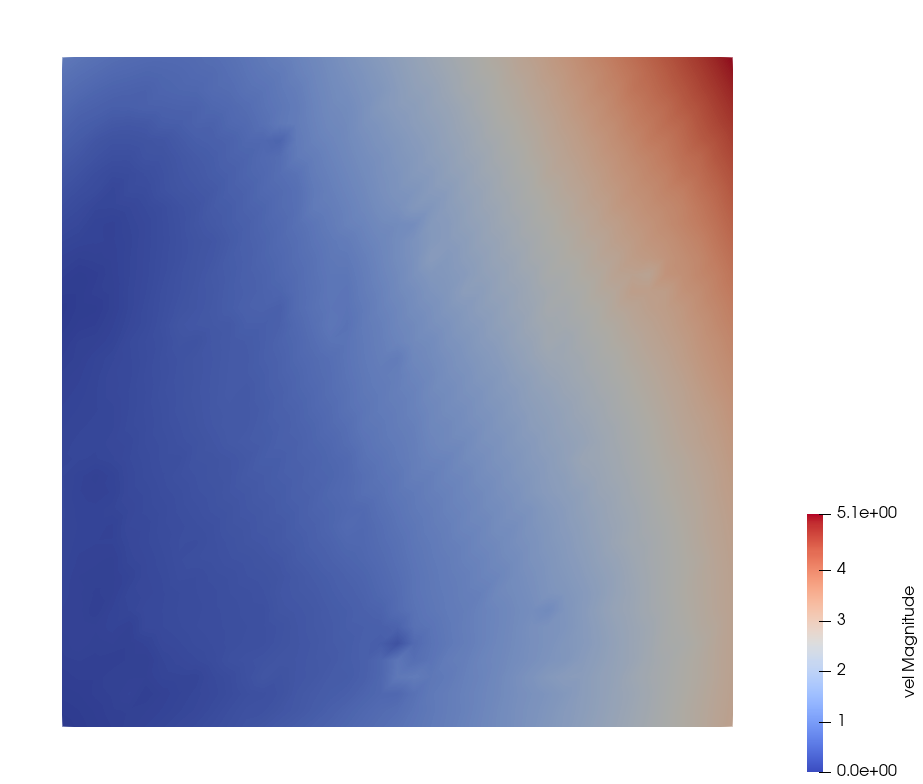
\includegraphics[width=7cm]{../results/exp09/velpb.png}
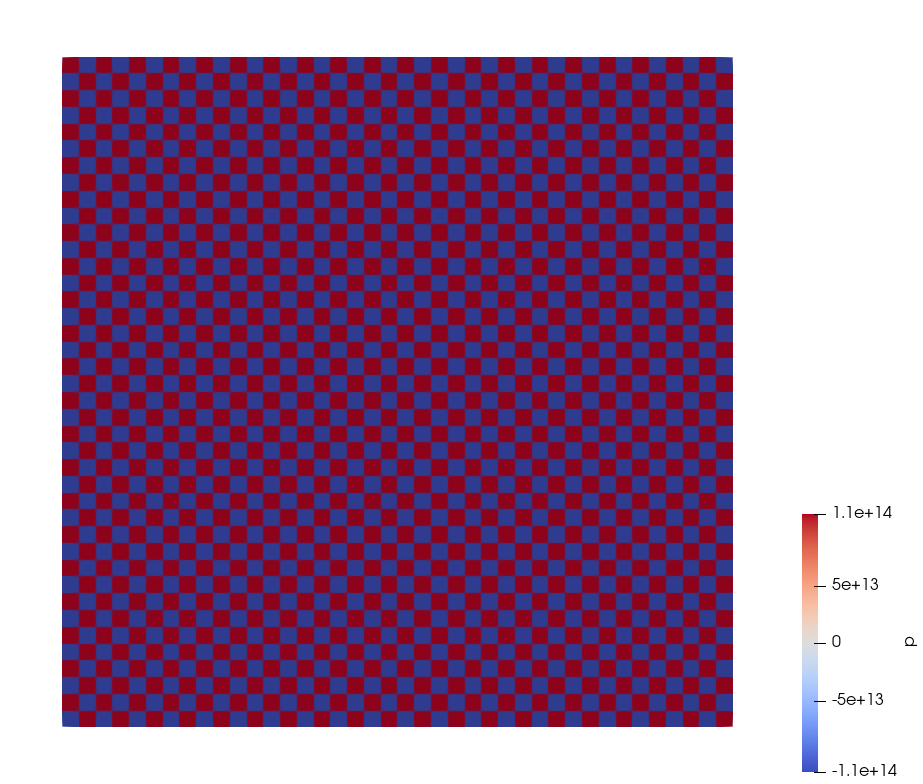
\includegraphics[width=7cm]{../results/exp09/presspb.png}
\end{center}

If I now run it by incorporating the constraint $\int_\Omega p dV = \sum_e A_e p_e$ in the 
matrix itself I find that the problem described above is completely absent, fields are smooth, 
rates are what is expected, comparable to D\&H benchmark. 

I *suspect* that this behavior could be due to the fact that for once a manufactured solution 
does not rely on no-slip b.c. and may be there is some kind of imbalance in the overal (discrete)
flux (flow is incompressible, we should have $\int_\Gamma \vec{u}\cdot\vec{n}d\Gamma=0$) 
and therefore triggers insane pressure oscillations and 
yields the problem above? and my instinct then tells me that 
by adding this extra line (and corresponding column) of constraints in the matrix it somewhat 
introduces some 'wiggle room' (\#technicalterm:) that compensates for the error in the b.c. imposition?
 
Am I in the right direction? if so could you put some maths around this? 
If not, any idea what causes the pb, or the solution? :)
 







